\documentclass[
  man,
  floatsintext,
  longtable,
  nolmodern,
  notxfonts,
  notimes,
  colorlinks=true,linkcolor=blue,citecolor=blue,urlcolor=blue]{apa7}

\usepackage{amsmath}
\usepackage{amssymb}



\usepackage[bidi=default]{babel}
\babelprovide[main,import]{english}


% get rid of language-specific shorthands (see #6817):
\let\LanguageShortHands\languageshorthands
\def\languageshorthands#1{}

\RequirePackage{longtable}
\RequirePackage{threeparttablex}

\makeatletter
\renewcommand{\paragraph}{\@startsection{paragraph}{4}{\parindent}%
	{0\baselineskip \@plus 0.2ex \@minus 0.2ex}%
	{-.5em}%
	{\normalfont\normalsize\bfseries\typesectitle}}

\renewcommand{\subparagraph}[1]{\@startsection{subparagraph}{5}{0.5em}%
	{0\baselineskip \@plus 0.2ex \@minus 0.2ex}%
	{-\z@\relax}%
	{\normalfont\normalsize\bfseries\itshape\hspace{\parindent}{#1}\textit{\addperi}}{\relax}}
\makeatother




\usepackage{longtable, booktabs, multirow, multicol, colortbl, hhline, caption, array, float, xpatch}
\setcounter{topnumber}{2}
\setcounter{bottomnumber}{2}
\setcounter{totalnumber}{4}
\renewcommand{\topfraction}{0.85}
\renewcommand{\bottomfraction}{0.85}
\renewcommand{\textfraction}{0.15}
\renewcommand{\floatpagefraction}{0.7}

\usepackage{tcolorbox}
\tcbuselibrary{listings,theorems, breakable, skins}
\usepackage{fontawesome5}

\definecolor{quarto-callout-color}{HTML}{909090}
\definecolor{quarto-callout-note-color}{HTML}{0758E5}
\definecolor{quarto-callout-important-color}{HTML}{CC1914}
\definecolor{quarto-callout-warning-color}{HTML}{EB9113}
\definecolor{quarto-callout-tip-color}{HTML}{00A047}
\definecolor{quarto-callout-caution-color}{HTML}{FC5300}
\definecolor{quarto-callout-color-frame}{HTML}{ACACAC}
\definecolor{quarto-callout-note-color-frame}{HTML}{4582EC}
\definecolor{quarto-callout-important-color-frame}{HTML}{D9534F}
\definecolor{quarto-callout-warning-color-frame}{HTML}{F0AD4E}
\definecolor{quarto-callout-tip-color-frame}{HTML}{02B875}
\definecolor{quarto-callout-caution-color-frame}{HTML}{FD7E14}

%\newlength\Oldarrayrulewidth
%\newlength\Oldtabcolsep


\usepackage{hyperref}




\providecommand{\tightlist}{%
  \setlength{\itemsep}{0pt}\setlength{\parskip}{0pt}}
\usepackage{longtable,booktabs,array}
\usepackage{calc} % for calculating minipage widths
% Correct order of tables after \paragraph or \subparagraph
\usepackage{etoolbox}
\makeatletter
\patchcmd\longtable{\par}{\if@noskipsec\mbox{}\fi\par}{}{}
\makeatother
% Allow footnotes in longtable head/foot
\IfFileExists{footnotehyper.sty}{\usepackage{footnotehyper}}{\usepackage{footnote}}
\makesavenoteenv{longtable}

\usepackage{graphicx}
\makeatletter
\def\maxwidth{\ifdim\Gin@nat@width>\linewidth\linewidth\else\Gin@nat@width\fi}
\def\maxheight{\ifdim\Gin@nat@height>\textheight\textheight\else\Gin@nat@height\fi}
\makeatother
% Scale images if necessary, so that they will not overflow the page
% margins by default, and it is still possible to overwrite the defaults
% using explicit options in \includegraphics[width, height, ...]{}
\setkeys{Gin}{width=\maxwidth,height=\maxheight,keepaspectratio}
% Set default figure placement to htbp
\makeatletter
\def\fps@figure{htbp}
\makeatother


% definitions for citeproc citations
\NewDocumentCommand\citeproctext{}{}
\NewDocumentCommand\citeproc{mm}{%
  \begingroup\def\citeproctext{#2}\cite{#1}\endgroup}
\makeatletter
 % allow citations to break across lines
 \let\@cite@ofmt\@firstofone
 % avoid brackets around text for \cite:
 \def\@biblabel#1{}
 \def\@cite#1#2{{#1\if@tempswa , #2\fi}}
\makeatother
\newlength{\cslhangindent}
\setlength{\cslhangindent}{1.5em}
\newlength{\csllabelwidth}
\setlength{\csllabelwidth}{3em}
\newenvironment{CSLReferences}[2] % #1 hanging-indent, #2 entry-spacing
 {\begin{list}{}{%
  \setlength{\itemindent}{0pt}
  \setlength{\leftmargin}{0pt}
  \setlength{\parsep}{0pt}
  % turn on hanging indent if param 1 is 1
  \ifodd #1
   \setlength{\leftmargin}{\cslhangindent}
   \setlength{\itemindent}{-1\cslhangindent}
  \fi
  % set entry spacing
  \setlength{\itemsep}{#2\baselineskip}}}
 {\end{list}}
\usepackage{calc}
\newcommand{\CSLBlock}[1]{\hfill\break\parbox[t]{\linewidth}{\strut\ignorespaces#1\strut}}
\newcommand{\CSLLeftMargin}[1]{\parbox[t]{\csllabelwidth}{\strut#1\strut}}
\newcommand{\CSLRightInline}[1]{\parbox[t]{\linewidth - \csllabelwidth}{\strut#1\strut}}
\newcommand{\CSLIndent}[1]{\hspace{\cslhangindent}#1}


\usepackage[nolongtablepatch]{lineno}
\linenumbers



\usepackage{newtx}

\defaultfontfeatures{Scale=MatchLowercase}
\defaultfontfeatures[\rmfamily]{Ligatures=TeX,Scale=1}





\title{Meta-analysis of the Interoceptive Accuracy Scale (IAS) Structure
and its Subjective Correlates}


\shorttitle{IAS Meta-analysis}


\usepackage{etoolbox}






\author{Ana Neves}



\affiliation{
{School of Psychology, University of Sussex}}




\leftheader{Neves}



\abstract{Blabla the abstract blabla.}

\keywords{keyword1, keyword2, keyword3}

\authornote{\par{\addORCIDlink{Ana Neves}{0009-0006-0020-7599}} 

\par{     \begin{tcolorbox}[enhanced jigsaw, breakable, bottomrule=.15mm, rightrule=.15mm, toprule=.15mm, left=2mm, colback=white, arc=.35mm, colframe=quarto-callout-note-color-frame, leftrule=.75mm, opacityback=0]

\end{tcolorbox}

This preprint is a non-peer-reviewed work from the
\href{https://realitybending.github.io/}{\textbf{Reality Bending Lab}}.
\begin{center}

\includegraphics[width=0.2\textwidth,height=\textheight]{manuscript_files/mediabag/ReBeL_LogoOnly_hu114.png}
\end{center}  Author roles were classified using the Contributor Role Taxonomy (CRediT; https://credit.niso.org/) as follows: Ana
Neves:   Project administration, Data curation, Formal
Analysis, Investigation, Visualization, Writing -- original
draft, Writing -- review \& editing}
\par{Correspondence concerning this article should be addressed to }
}

\makeatletter
\let\endoldlt\endlongtable
\def\endlongtable{
\hline
\endoldlt
}
\makeatother

\urlstyle{same}



\usepackage{lscape}
\makeatletter
\@ifpackageloaded{tcolorbox}{}{\usepackage[skins,breakable]{tcolorbox}}
\@ifpackageloaded{fontawesome5}{}{\usepackage{fontawesome5}}
\definecolor{quarto-callout-color}{HTML}{909090}
\definecolor{quarto-callout-note-color}{HTML}{0758E5}
\definecolor{quarto-callout-important-color}{HTML}{CC1914}
\definecolor{quarto-callout-warning-color}{HTML}{EB9113}
\definecolor{quarto-callout-tip-color}{HTML}{00A047}
\definecolor{quarto-callout-caution-color}{HTML}{FC5300}
\definecolor{quarto-callout-color-frame}{HTML}{acacac}
\definecolor{quarto-callout-note-color-frame}{HTML}{4582ec}
\definecolor{quarto-callout-important-color-frame}{HTML}{d9534f}
\definecolor{quarto-callout-warning-color-frame}{HTML}{f0ad4e}
\definecolor{quarto-callout-tip-color-frame}{HTML}{02b875}
\definecolor{quarto-callout-caution-color-frame}{HTML}{fd7e14}
\makeatother
\makeatletter
\@ifpackageloaded{caption}{}{\usepackage{caption}}
\AtBeginDocument{%
\ifdefined\contentsname
  \renewcommand*\contentsname{Table of contents}
\else
  \newcommand\contentsname{Table of contents}
\fi
\ifdefined\listfigurename
  \renewcommand*\listfigurename{List of Figures}
\else
  \newcommand\listfigurename{List of Figures}
\fi
\ifdefined\listtablename
  \renewcommand*\listtablename{List of Tables}
\else
  \newcommand\listtablename{List of Tables}
\fi
\ifdefined\figurename
  \renewcommand*\figurename{Figure}
\else
  \newcommand\figurename{Figure}
\fi
\ifdefined\tablename
  \renewcommand*\tablename{Table}
\else
  \newcommand\tablename{Table}
\fi
}
\@ifpackageloaded{float}{}{\usepackage{float}}
\floatstyle{ruled}
\@ifundefined{c@chapter}{\newfloat{codelisting}{h}{lop}}{\newfloat{codelisting}{h}{lop}[chapter]}
\floatname{codelisting}{Listing}
\newcommand*\listoflistings{\listof{codelisting}{List of Listings}}
\makeatother
\makeatletter
\makeatother
\makeatletter
\@ifpackageloaded{caption}{}{\usepackage{caption}}
\@ifpackageloaded{subcaption}{}{\usepackage{subcaption}}
\makeatother

% From https://tex.stackexchange.com/a/645996/211326
%%% apa7 doesn't want to add appendix section titles in the toc
%%% let's make it do it
\makeatletter
\xpatchcmd{\appendix}
  {\par}
  {\addcontentsline{toc}{section}{\@currentlabelname}\par}
  {}{}
\makeatother

%% Disable longtable counter
%% https://tex.stackexchange.com/a/248395/211326

\usepackage{etoolbox}

\makeatletter
\patchcmd{\LT@caption}
  {\bgroup}
  {\bgroup\global\LTpatch@captiontrue}
  {}{}
\patchcmd{\longtable}
  {\par}
  {\par\global\LTpatch@captionfalse}
  {}{}
\apptocmd{\endlongtable}
  {\ifLTpatch@caption\else\addtocounter{table}{-1}\fi}
  {}{}
\newif\ifLTpatch@caption
\makeatother

\begin{document}

\maketitle


\setcounter{secnumdepth}{-\maxdimen} % remove section numbering

\setlength\LTleft{0pt}

\resetlinenumber[1]

Interoception is referred to the process of sensing, interpreting and
integrating information pertaining to internal organs, such as the
heart, the lungs or the gut (\citeproc{ref-khalsa2018}{Khalsa et al.,
2018}). While recent research emphasizes a key role of interoception in
a variety of processes (e.g., emotion regulation, decision making) and
of outcomes (physical and psychological well being), the field remains
clouded by concerns about how interoception is assessed.

Various measures of interoception have been developed (see
\textbf{Figure~\ref{fig-measures}}), forming a combination of
``objective'' and ``subjective'' assessments (i.e., physiological tasks
such as the heart beat counting or tracking vs.~questionnaires and
subjective scales involving a metacognitive reflection), ``explicit''
and ``implicit'' paradigms (i.e., directing participants' awareness and
attention to interoceptive processes \emph{vs.} measuring interoception
unbeknownst to them), various interoceptive modalities (e.g.,
cardioception, respiroception, gastroception) and theoretical dimensions
(e.g., accuracy, sensitivity, awareness). While there is no consensus as
to which particular approach provides the most accurate and ``pure''
measure of interoception and interoceptive abilities (assuming it is a
unidimensional construct), it is instead plausible that each measure has
strengths and limitations, and a utility dependent on the context and
goal at hand (\citeproc{ref-jahedi2014}{Jahedi \& Méndez, 2014}).

\begin{figure*}[!htbp]

{\caption{{Different ways in which interoception can be
measured.}{\label{fig-measures}}}}

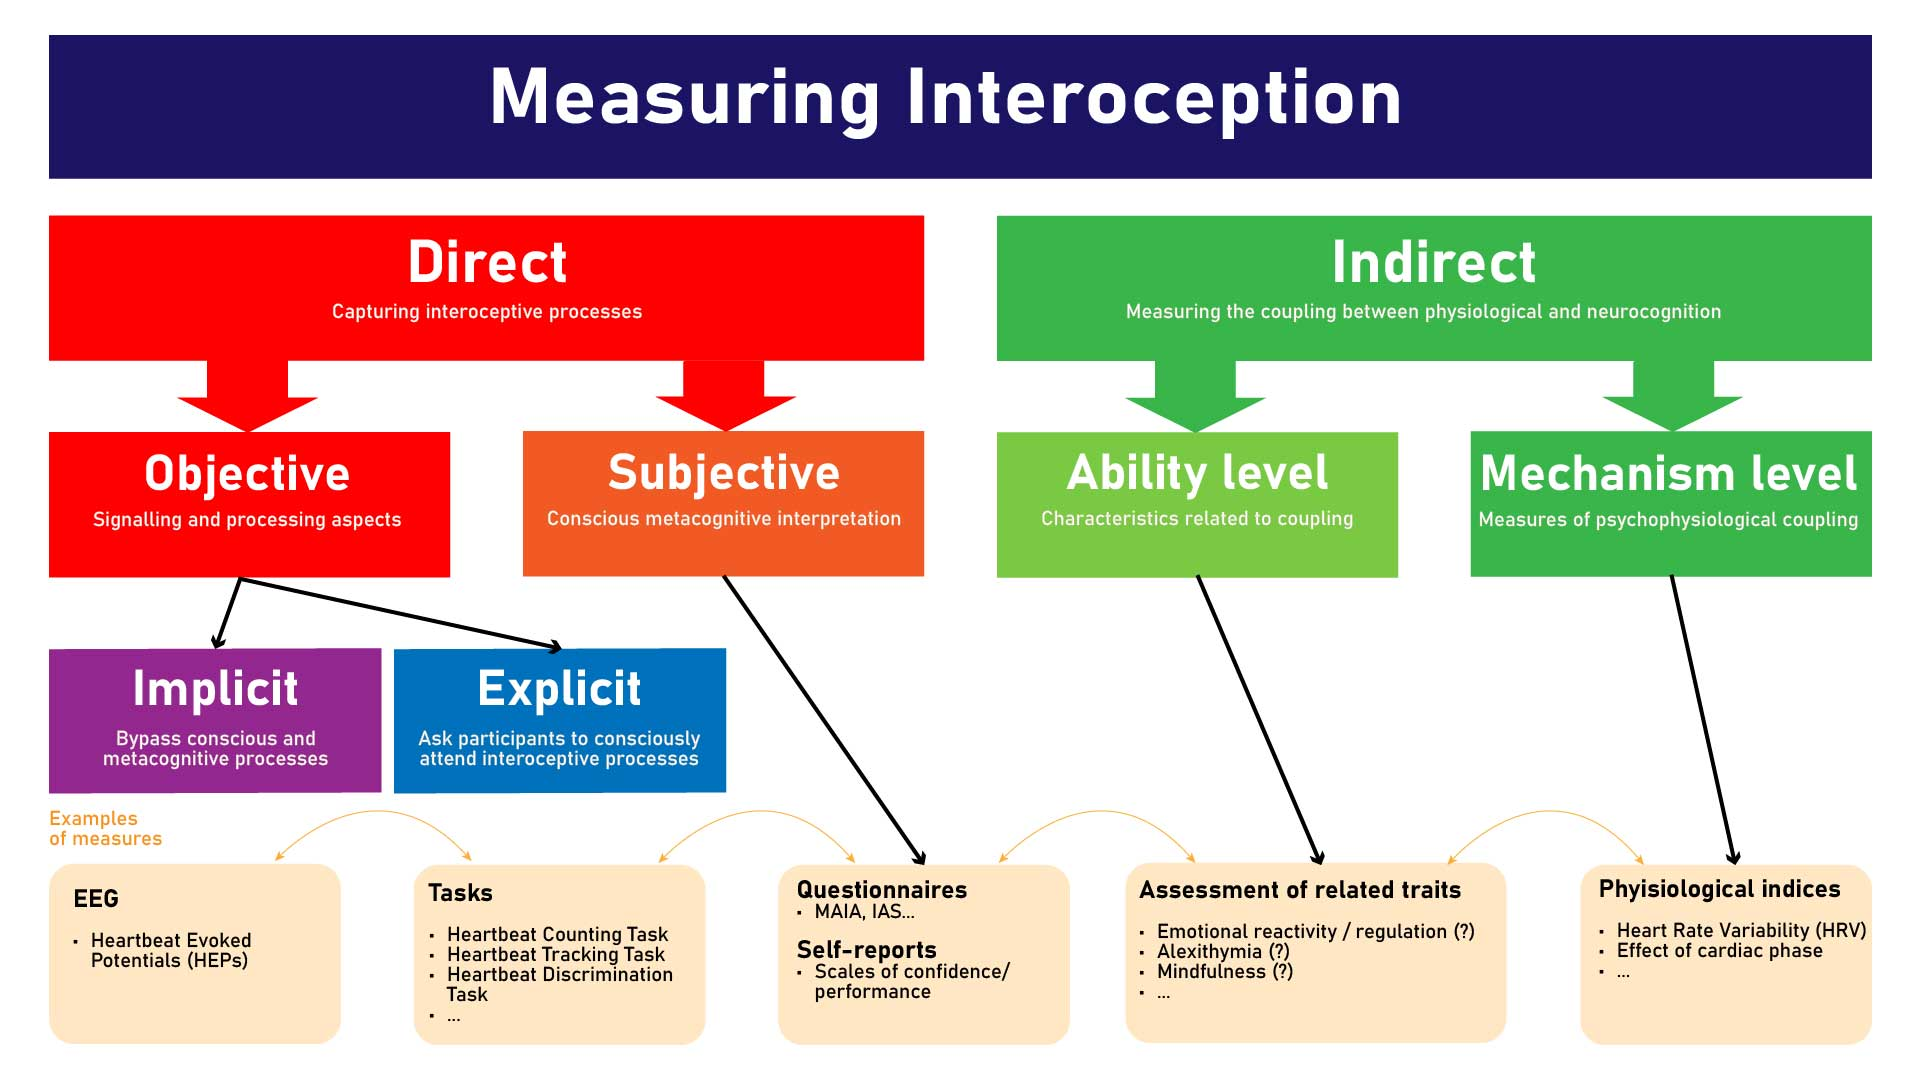
\includegraphics[width=1\textwidth,height=\textheight]{figures/MeasuringInteroception.jpg}

\end{figure*}

The use of subjective self-report questionnaires to measure deeply
embodied functions might seem paradoxical. However, recent redefinitions
of interoception emphasize the role of high-level and metacognitive
elaboration of interoceptive information. These redefinitions provide
theoretical grounding to support the idea that some facets of
interoception, including participants' metacognitive beliefs, can be
assessed subjectively. This approach offers useful and interesting
measures (\citeproc{ref-lin2023}{Lin et al., 2023};
\citeproc{ref-murphy2019}{Murphy et al., 2019}).

The notion that self-reports might not reflect the same processes as
other interoception measures is important to contextualize the apparent
lack of convergence between measures in the field
(\citeproc{ref-desmedt2022measures}{Desmedt et al., 2022}).

A recent systematic review by Desmedt et al.
(\citeproc{ref-desmedt2022measures}{2022}) examined whether various
questionnaires designed to measure ``interoceptive sensibility'' truly
assess the same construct. Notably, Garfinkel et al.
(\citeproc{ref-garfinkel2015knowing}{2015}) defines interoceptive
sensibility as the self-reported tendency to focus on and detect
internal sensations, whereas
(\citeproc{ref-khalsa2018interoception}{\textbf{khalsa2018interoception?}})
defines it more narrowly, excluding the ability to detect these signals.
According to Desmedt et al. (\citeproc{ref-desmedt2022measures}{2022}),
most authors adopt the latter definition. The review found that these
questionnaires measure related but distinct constructs, leading
researchers to commit the `jingle fallacy'---mistakenly treating them as
equivalent measures of interoceptive sensibility.

\textbf{TODO: do a better job}

Few studies have examined the correlation between objective
interoceptive measures, such as the Heartbeat Counting Task (HCT;
Schandry, 1981) and the Heartbeat Detection Task (HDT; Kleckner et al.,
2015). Existing findings report weak correlations for the HCT (Murphy et
al., 2019), no correlations except for the sensitivity variable of the
HCT (Brand et al., 2023), and small correlations for the HDT (Brand et
al., 2023). These results suggest that the IAS, a subjective measure,
does not strongly align with objective interoceptive assessments.

A better understanding of what is being measured with different
questionnaires and dimensions, as well as their potential overlaps with
other constructs (e.g., alexithymia, body awareness), is thus needed to
clarify the role of self-reports in the assessment of interoception.

A recently developed scale with a rapidly growing popularity is the
Interoceptive Accuracy Scale (IAS, \citeproc{ref-murphy2019}{Murphy et
al., 2019}). The IAS consists of 21 Likert-scale items that query how
accurately one can perceive different bodily signals, with one item per
physiological modality such as respiration (\emph{``I can always
accurately perceive when I am breathing fast''}), heart (e.g \emph{``I
can always accurately perceive when my heart is beating fast''}), skin
(e.g \emph{``I can always accurately perceive when something is going to
be ticklish''}), arousal or bodily functions like coughing (e.g
\emph{``I can always accurately perceive when I am going to cough''}) or
urinating (e.g.~\emph{``I can always accurately perceive when I need to
urinate''}). Interestingly, the IAS' statements are about specific
interoceptive behaviours, which is a notable difference with other
popular interoception questionnaires, such as the Multidimensional
Assessment of Interoceptive Awareness scale (MAIA,
\citeproc{ref-mehling2012}{Mehling et al., 2012}; MAIA-2,
\citeproc{ref-mehling2018multidimensional}{Mehling et al., 2018}), which
contains more general and metacognitive items (e.g., \emph{``I trust my
body sensations''}, \emph{``I can notice an unpleasant body sensation
without worrying about it''}).

Although the original validation study suggested a two-factor structure
for the IAS, the authors underline its acceptable but imperfect fit
{[}Murphy et al. (\citeproc{ref-murphy2019}{2019}); p.~127{]}, calling
on further investigation of the scale's factor structure. Notably, the
authors did not define these factors, as no clear explanations were
evident. They suggested that the first factor reflects the perception of
interoceptive signals, while the second pertains to signals that may be
difficult to perceive solely through interoceptive information.

Other follow-up studies using confirmatory factor analysis (CFA) and
structural modeling have identified different optimal solutions. Some
studies, like Brand et al. (\citeproc{ref-brand2023}{2023}), reported a
1-factor solution, while Lin et al. (\citeproc{ref-lin2023}{2023}) and
Campos et al. (\citeproc{ref-campos2021}{2021}) found bifactor solutions
- one general factor and a set of lower-level factors
(\citeproc{ref-rodriguez2016evaluating}{Rodriguez et al., 2016}) - to be
the best fit. Notably, the only other study to report a 2-factor
solution was conducted by Koike and Nomura
(\citeproc{ref-koike2023}{2023}), who performed an Exploratory Factor
Analysis (EFA) assuming 2 factors to align with the findings from the
original validation paper.

Discussions have also been focused on specific items. For instance,
Murphy et al. (\citeproc{ref-murphy2019}{2019}) notes that some items
might measure direct interoceptive signals such as cardioception, while
others might capture phenomena not perceivable through interoceptive
signals alone (e.g., ``bruising''; p.~119). Lin et al.
(\citeproc{ref-lin2023}{2023}) also highlights their correlation
analysis, showing five locally dependent pairs and three items (touch,
blood sugar, bruise) with exceptionally high difficulty and low
discrimination. Additionally, Campos et al.
(\citeproc{ref-campos2021}{2021}) reported ``tickle'' to be the only
item that reflected more specific factors than the general factor.
Interestingly, Lin et al. (\citeproc{ref-lin2023}{2023}) reported that
all items of the IAS grouped together using a new approach, Exploratory
Graph Analysis {[}EGA; Golino and Epskamp
(\citeproc{ref-golino2017exploratory}{2017}){]}, to assess convergent
and discriminant validity, providing further evidence for
unidimensionality.

The IAS has naturally been compared to other interoception-related
scales, and shows a positive correlations with most facets of the MAIA
(\citeproc{ref-mehling2018multidimensional}{Mehling et al., 2018}),
except for the Non-Distracting and Not-Worrying subscales
(\citeproc{ref-brand2023}{Brand et al., 2023}). Interestingly, findings
on the correlation between the IAS and the body awareness dimension of
the Body Perception Questionnaire (BPQ-A,
\citeproc{ref-porges1993body}{Porges, 1993}) have been mixed: some
studies report small positive correlations
(\citeproc{ref-brand2023}{Brand et al., 2023};
\citeproc{ref-campos2021}{Campos et al., 2021};
\citeproc{ref-koike2023}{Koike \& Nomura, 2023}), while others find
small negative correlations (\citeproc{ref-lin2023}{Lin et al., 2023})
or no correlation at all (\citeproc{ref-murphy2019}{Murphy et al.,
2019}). Small positive correlations have also been observed with the
``observation'' and ``description'' subscales of the Five Facet
Mindfulness Questionnaire (FFMQ, \citeproc{ref-baer2006using}{Baer et
al., 2006}; \citeproc{ref-brand2023}{Brand et al., 2023};
\citeproc{ref-koike2023}{Koike \& Nomura, 2023}), as well as with the
``non-reactivity'' and ``acting with awareness'' subscales
(\citeproc{ref-koike2023}{Koike \& Nomura, 2023}). Additionally, the IAS
has shown a positive correlation with the interoceptive awareness
subscale of the Eating Disorder Inventory (\citeproc{ref-lin2023}{Lin et
al., 2023}) and a negative correlation with the Interoceptive Confusion
Questionnaire (\citeproc{ref-brand2023}{Brand et al., 2023}; ICQ,
\citeproc{ref-brewer2016alexithymia}{Brewer et al., 2016};
\citeproc{ref-murphy2019}{Murphy et al., 2019}). Lastly, small positive
correlations have also been reported with the Interoceptive Attention
Scale (\citeproc{ref-koike2023}{Koike \& Nomura, 2023}; IATS,
\citeproc{ref-lin2023}{Lin et al., 2023}), though studies have also
found no correlation between these measures
(\citeproc{ref-gabriele2022dissociations}{Gabriele et al., 2022}).

While assessing the validity of an interoception scale can be conceived
as theoretically challenging, several measures have been used to assess
convergent validity for the the IAS, including expected negative
associations with alexithymia Murphy et al.
(\citeproc{ref-murphy2019}{2019}), somatic symptoms Lin et al.
(\citeproc{ref-lin2023}{2023}), depressive symptoms
(\citeproc{ref-brand2023}{Brand et al., 2023};
\citeproc{ref-koike2023}{Koike \& Nomura, 2023};
\citeproc{ref-lin2023}{Lin et al., 2023}), anxiety
(\citeproc{ref-brand2023}{Brand et al., 2023}), neuroticism
(\citeproc{ref-brand2023}{Brand et al., 2023}) and self-esteem
(\citeproc{ref-murphy2019}{Murphy et al., 2019}).

The current study aims at 1) clarifying the structure of the IAS with a
meta-analytic approach that leverages existing data and contrast the
traditional CFA/SEM factor-based analyses with network-based ones such
as EGA. 2) The second part will provide an overview of the dispositional
correlates of the IAS, providing an overview of the pattern of
associations that is key to better understand the nature, place and role
of interoception questionnaires within a larger context.

\subsection{Study 1}\label{study-1}

The goal of study 1 is to re-analyse and assess the factor structure of
the IAS by taking advantage of the large number of open-access datasets
(\citeproc{ref-arslanova2022}{Arslanova et al., 2022};
\citeproc{ref-brand2022}{Brand et al., 2022};
\citeproc{ref-brand2023}{Brand et al., 2023};
\citeproc{ref-campos2021}{Campos et al., 2021};
\citeproc{ref-gaggero2021}{Gaggero et al., 2021};
\citeproc{ref-lin2023}{Lin et al., 2023};
\citeproc{ref-murphy2019}{Murphy et al., 2019};
\citeproc{ref-todd2022}{Todd et al., 2022}; \citeproc{ref-von2023}{Von
Mohr et al., 2023}). While combining these studies might provide a more
robust and generalizable understanding of the IAS' factor structure, we
also additionally provide an individual analysis (i.e., on all samples
separately) to add nuance to the general picture, as all studies differ
in their sample sizes, demographics, language, and procedure.

\subsubsection{Methods}\label{methods}

\paragraph{Datasets.}\label{datasets}

Our search focused on studies citing the original IAS validation paper
(\citeproc{ref-murphy2019}{Murphy et al., 2019}), identifying 136 papers
(as of 01/05/2024). To qualify for inclusion, papers needed to (1)
provide accessible data in open-access, (2) employ the IAS as a measure,
and (3) report individual IAS items scores. A total of 10 studies was
included (see \textbf{Table 1}). We also included the data of two
unpublished (but already open-access) studies from the authors and one
from another author. The total N participants was 32,214 participants
(\emph{Mean} = 48.6 years, \emph{SD} = 13.1, 71.6\% Female).

\paragraph{Statistical Analysis.}\label{statistical-analysis}

To examine the factor structure of the IAS, a two-step approach was
employed. First, Exploratory Graph Analysis (EGA), was used to estimate
the dimensions via network estimation and community detection, alongside
assessing the stability of dimensions and items using the bootstrapping
techniques (\citeproc{ref-golino2017exploratory}{Golino \& Epskamp,
2017}). The selection of EGA was motivated by its capability to handle
complex, multidimensional data and provide robust dimension estimates. A
novel network psychometrics - Unique variable analysis {[}UVA;
Christensen et al. (\citeproc{ref-christensen2023unique}{2023}){]} -
approach based on the weighted topological overlap will be computed to
evaluate which items have substantial local dependence (\textgreater{}
0.25). Subsequently, exploratory factor analysis (EFA) was employed
followed by confirmatory factor analysis (CFA).

\subsubsection{Results}\label{results}

Visualizing the distribution of the items for all samples suggests the
presence of a consistent modal value (Figure~\ref{fig-distributions}).
In other words, participants are most likely to answer 4/5 (i.e., agree)
on most items (but ``affective touch'', ``blood sugar'', and ``bruise''
that exhibit a different distributional pattern). Additionally, one can
note the low density on extreme values (1 and 5), meaning that the bulk
of answers (i.e., 99\%) varies between 3 values. The interindividual
variability seems improved in the samples using an analogue scale,
displaying a more continuous and progressive spread of answers.

\begin{figure}

\caption{\label{fig-distributions}Distribution of responses for all
items across various datasets.}

\centering{

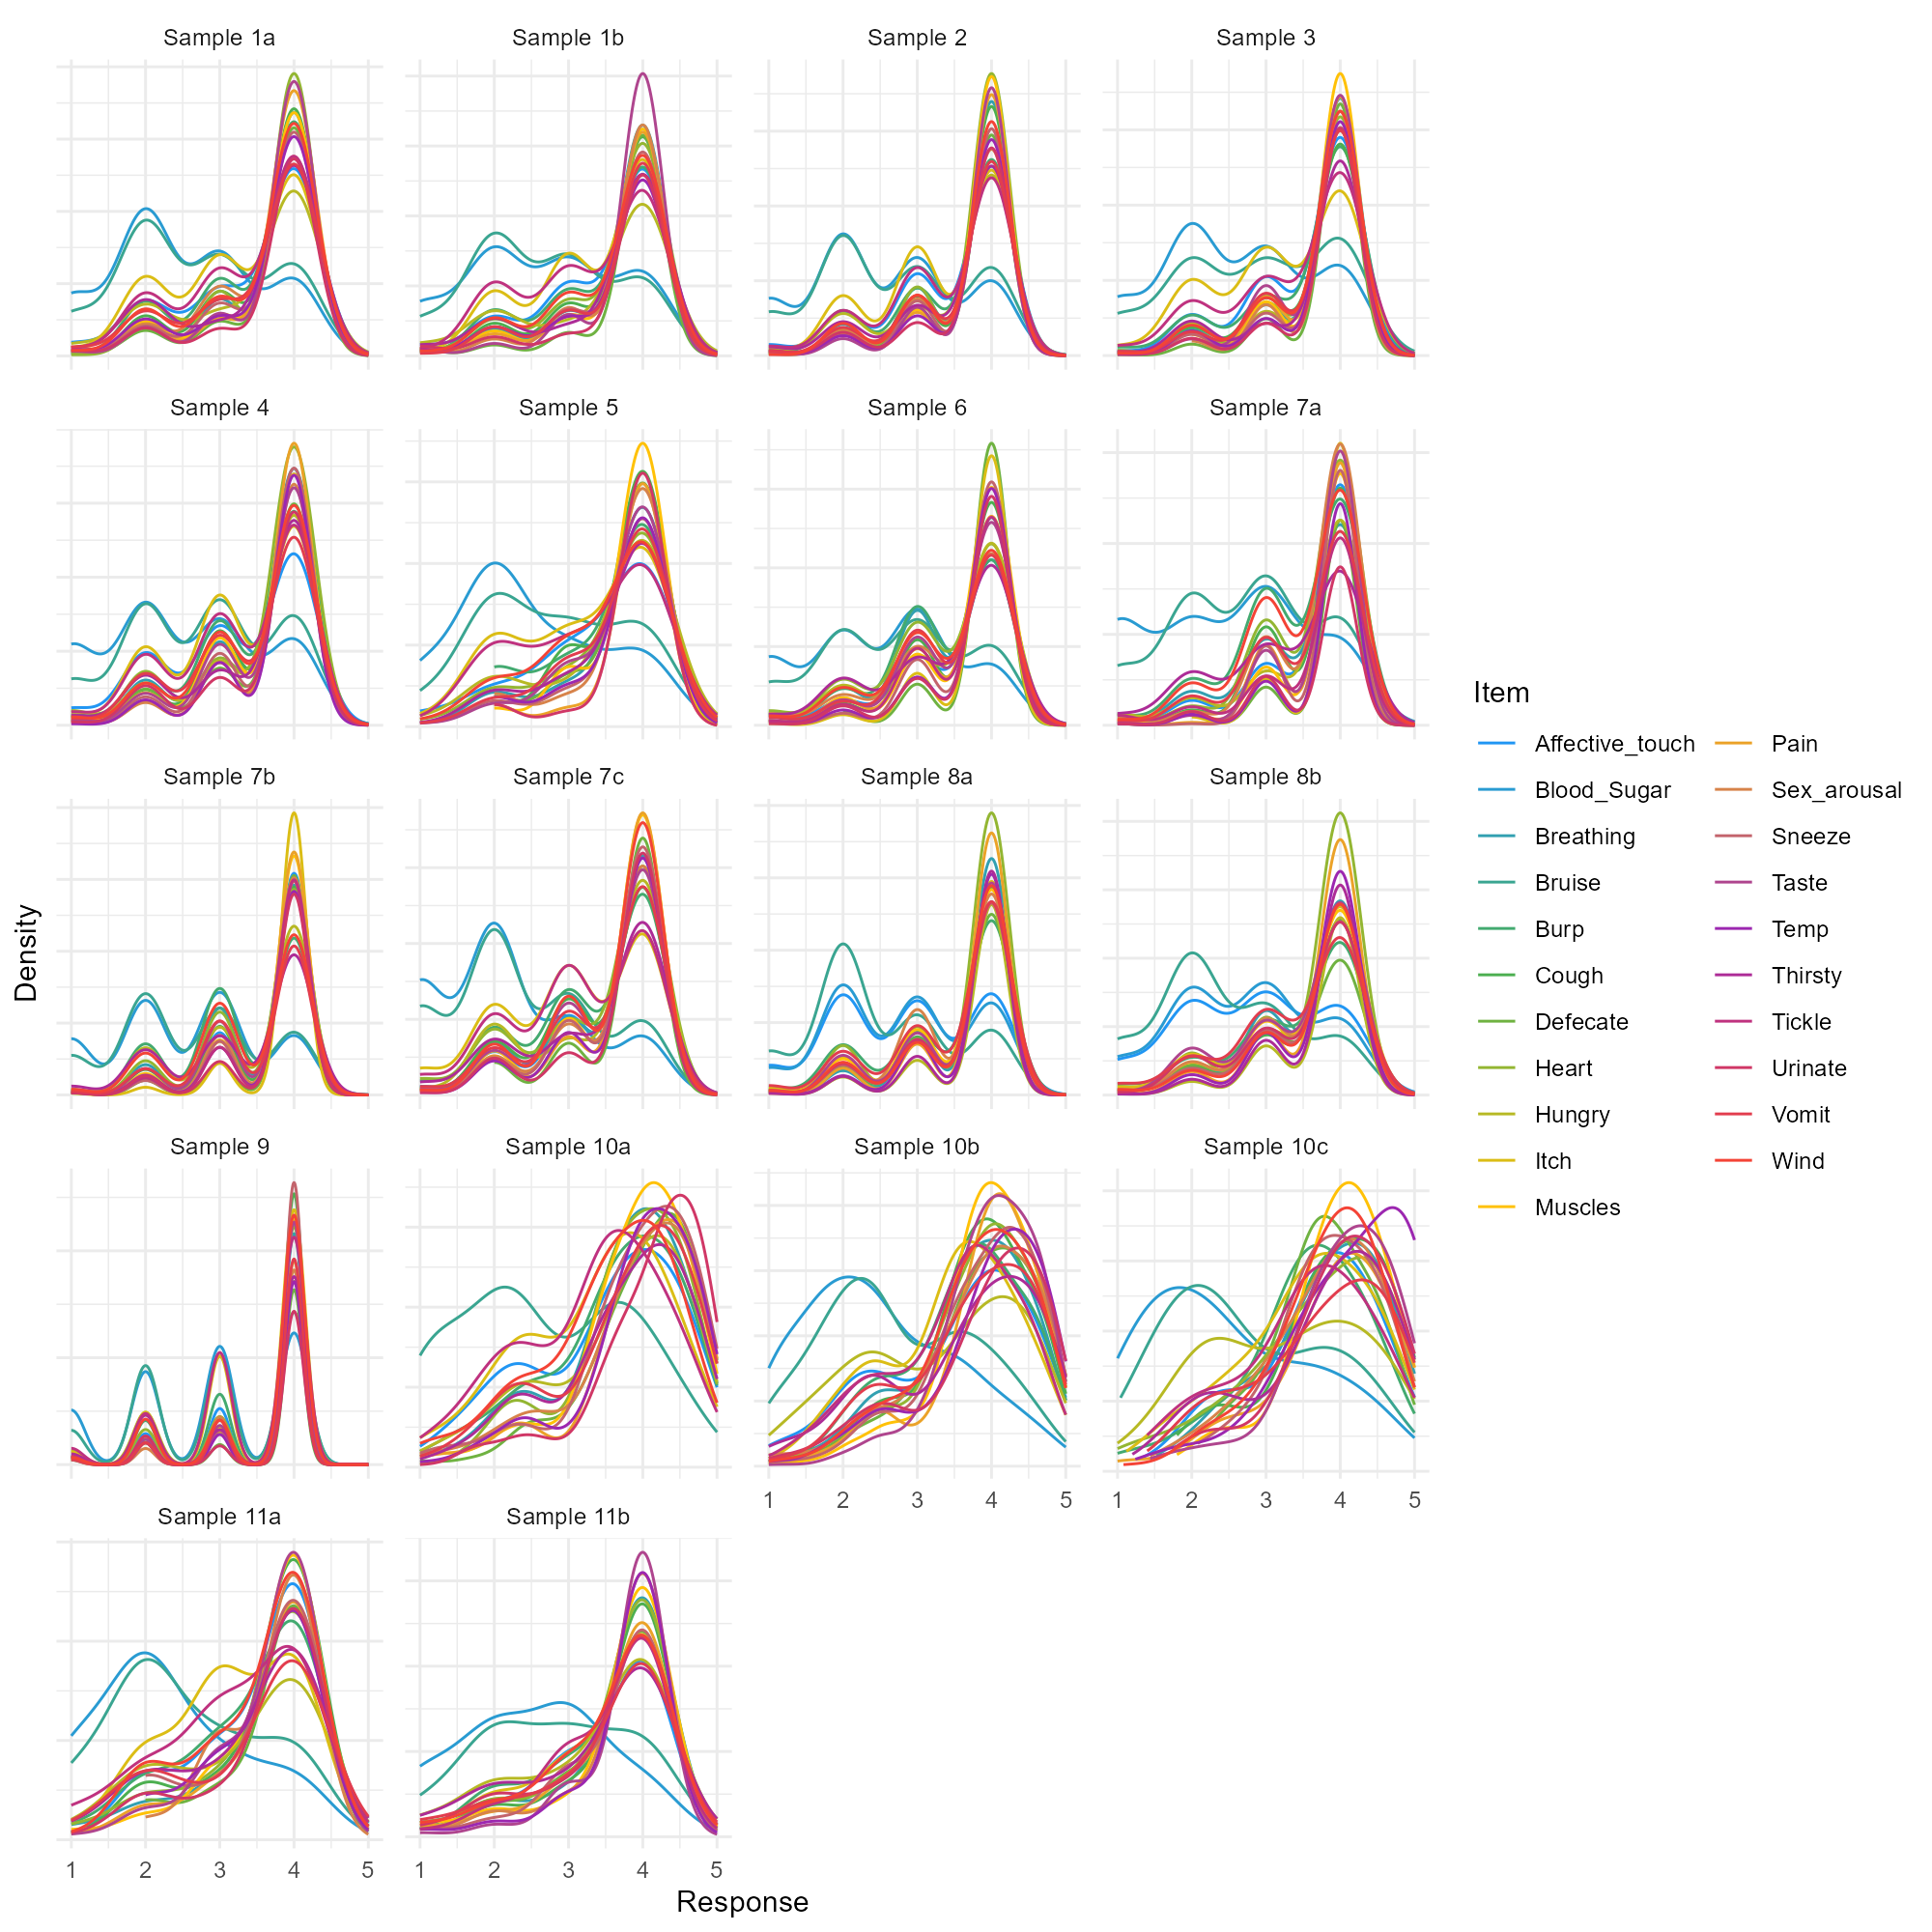
\includegraphics[width=6.67in,height=\textheight]{figures/Figure1.png}

}

\end{figure}%

\paragraph{Correlations.}\label{correlations}

The correlation analysis revealed that the items overall have positive
intercorrelation patterns with no clear structure emerging. This remains
the same across all samples. However, there are possibly some
higher-order groupings emerging for the 2 analog-scale samples.

\paragraph{EGA.}\label{ega}

The UVA revealed that there are two large to very large redundant
variables when taking all samples into account. Namely, ``itch'' and
``tickle'', where ``tickle'' should be removed, and ``itch'' should be
kept. There are several more items that are moderately to largely
redundant, namely, ``wind'' and ``burp'', and ``urinate'' and
``defecate''. On top of that, ``sneeze'' and ``cough'', ``heart'' and
``breathing'', and ``hungry'' and ``thirsty'' seem to have small to
moderate redundancy. These findings are rather consistent across the
samples with minor differences, such as that when the questionnaire had
an analog scale, there seems to be no large to very large redundant
items but ``itch'' and ``tickle'' remain moderately to largely redundant
and ``heart'' and ``breathing'' small to moderately redundant in one
sample.

According to the network analysis, using the Walktrap and Louvain
algorithms applied to Glasso networks, a 4-factor structure fits the
questionnaire best across all data sets. This is rather consistent
within the data sets, where some samples indicate 3-factor structure,
and some a 5-factor structure would fit well too. The 4-factor structure
model with the best fit entails the following items per group: 1) itch,
tickle, bruise, blood sugar; 2) burp, wind, cough, sneeze, vomit; 3)
affective touch, sexual arousal, muscles, temperature, pain, and taste;
4) Heart, breathing, hungry, thirsty, urinate, and defecate.

Stability analysis, employing 500 bootstrap iterations, also favoured
the 4-factor solution for its greater stability. Most items, except for
`affective touch,' demonstrated stability levels exceeding 0.90,
indicating structural consistency and reliability
(\citeproc{ref-christensen2021}{Christensen \& Golino, 2021}). These
findings underscore the robustness of the identified 4-dimensional
structure.

When accounting for all samples, the factor analysis reveals that a
4-factor structure fits best. The exploratory factor analysis revealed
that 4 latent factors (oblimin rotation) accounted for 51.95\% of the
total variance of the original data (MR2 = 19.08\%, MR1 = 17.78\%, MR4 =
9.34\%, MR3 = 5.75\%). Since UVA identified ``tickle'' as the item to be
removed---and it also had the lowest uniqueness value in factor analysis
with a similar loading to ``itch''---``tickle'' was excluded from
subsequent analyses.

Confirmatory factor analysis compared 5 models: a single-factor
solution, a 4-factor solution, a 5-factor solution, a 6-factor solution
and a 7-factor solution. The latter was preferred in most datasets,
including with indices that penalise increased number of parameters
(such as BIC). There was no evidence for higher order factors.

\subsubsection{Discussion}\label{discussion}

In this study, several datasets were analyzed for a meta analysis of the
structure of the IAS. The findings reveal that a 4-factor model fits the
IAS best. Additionally, the lowest level structure (pairs of items) seem
to be the most robust, especially for samples using Likert scales (some
higher-order groupings might emerge for the 2 analog-scale samples).
There was no clear evidence for higher-order factors.

These findings contrast with previous research, which all found that
2-factor model(\citeproc{ref-koike2023}{Koike \& Nomura, 2023};
\citeproc{ref-murphy2019}{Murphy et al., 2019}), 1-factor model
(\citeproc{ref-brand2023}{Brand et al., 2023}) and bifactor model
(\citeproc{ref-campos2021}{Campos et al., 2021};
\citeproc{ref-lin2023}{Lin et al., 2023}) fits the data best. While this
analysis also revealed an okay fit for the 1-factor model, the 4-factor
model revealed the best fit. The 4-factor structure reveals different
`hubs' of items that are related, not only in this structure analysis,
but also in underlying mechanisms. The `wind-burp-cough-sneeze-vomit'
category, for example, only entails items that are linked to excretion
through the mouth. The other categories are organized similarly. This
organization and structure is useful for further analysis, as the data
can be analyzed and interpreted according to a grouping that is coherent
in result, as well as underlying mechanisms.

There are several items that show redundancy suggesting that adapting
the IAS would be beneficial for validity. Based on the given results, we
suggest removing the tickle, while keeping the itch item
{[}\textbf{todo}: stats?{]}. Other items with slight redundancy were
Hungry and Thirsty, Urinate and Defecate, and Sneeze and Cough.

Interestingly, Lin et al. (\citeproc{ref-lin2023}{2023}) also found that
tickle and itch were redundant, excluding one of them but the reason
being that the character for both words is the same in the Chinese
language. On top of that, they came up with a shortened version of the
IAS, excluding further items, resulting in a 12-item IAS, which aligns
with our findings, suggesting that further items are ambiguous as to
whether they should be removed. In contrast, other findings also found
itch and tickle to be redundant but did not suggest excluding items
(\citeproc{ref-campos2021}{Campos et al., 2021}).

The findings indicate a high proportion of answers at 4 (see Figure 1),
especially when using a 5-step scale. The analogue scale shows a more
dispersed distribution, with some answers indicating the highest 5/5,
which was not the case in the 5-step scale. Therefore, we recommend
using an analog scale for the IAS.

Before this paper, the IAS has not yet been used or analyzed with an
analog scale, rather than a five step scale. Therefore, this study
provides a novel approach to improving the IAS in a simple manner.

\subsubsection{Limitations and Future
Directions}\label{limitations-and-future-directions}

There are several limitations to the IAS; There are some redundant
items, the 5-point scale does not provide great variability, and the
structure could be improved. Therefore, improving the IAS, or creating a
new questionnaire investigating interoception could be useful to
achieving reliable and accurate indication of interoceptive awareness.

\subsection{Study 2}\label{study-2}

Study 2 aims to investigate correlates of the IAS. Correlations of the
IAS will be computed to assess the relationship between subjective
interoceptive accuracy and other subjective measures of interoception,
mood, psychopathology, personality, and beliefs. Investigating
correlates will help validate the IAS, as well as other interoceptive
measures in the future. The

\subsubsection{Methods}\label{methods-1}

\paragraph{Materials.}\label{materials}

The questionnaires used for the IAS correlates are listed in
\textbf{Table 2} (\textbf{TODO: add the rest of the questionnaires,
sample items and references}).

\paragraph{Statistical analysis.}\label{statistical-analysis-1}

Correlations will be computed using the correlation package under a
Bayesian framework (ref).

\subsubsection{Results}\label{results-1}

\textbf{todo: compute average correlations }

The EGA components capture groupings of pairs of items, such as ``wind''
and ``burp'', ``cough'' and ``sneeze'', or ``muscle'' and ``pain''.
These groupings were used in the correlational analysis, to observe how
much each group/pair correlates with other factors, such as Alexithymia,
or the MAIA (see Figure 2).

Alexithymia is negatively correlated with all interoceptive groups.
Autistic traits are mostly negatively correlated with IAS measure,
except for patterns and numbers (as an autistic trait), which is
significantly and positively correlated with the ``itch/bruise''
pairing. The BPQ Body Awareness part is positively correlated with all
IAS pairs, whereas the Autonomic Reactivity part is negatively
correlated with all IAS groupings. Conspiracy Beliefs were all
positively correlated with the IAS pairs, however, only Global
Conspiracy with ``hungry/thirsty'', ``urinate/defecate'' and
``cough/sneeze'', as well as personal wellbeing with ``hungry/thirsty'',
and Information Control with ``cough/sneeze'' were significantly
positively correlated. Demographic data is also mostly positively
correlated with the IAS findings, where gender and age more strongly
correlated with ``hungry/thirsty''. In this analysis, lying profile is
not strongly correlated with the IAS; Except for contextuality, which
shows a significant negative correlation with ``itch/bruise''. The MAIA
has a strong positive correlation with most IAS pairings, except for the
``not worrying'' and ``not distracting'' items of the MAIA, which show
less strong, or even negative correlations with all IAS item pairings.
Maladaptiveness had mostly negative correlations with the IAS, with only
a few significant correlations, namely ``psychoticism'', ``negative
affect'', and ``detachment'' with ``muscle/pain'' and
``hungry/thirsty'', as well as ``negative affect'' with ``wind/burp''.
Overall, mood was mostly negatively correlated with the IAS, where
``hungry/thirsty'' had the strongest negative correlation of all mood
measures. Except for ``neuroticism'' and ``honesty-humility'',
personality traits, such as ``openness'' and ``extraversion'' were
positively correlated with the IAS groupings. Shizotypic traits were
mostly negatively correlated with the IAS, with ``hungry/thirsty''
showing the strongest negative correlation between schizotypic and the
IAS. World beliefs were mostly positively correlated with the IAS,
however, only a few were significant: ``hierarchical'', ``enticing'',
and ``alive'' correlates significantly with ``muscle/pain'';
``Understandable'' has a significant positive correlation with
``heart/breathing''; And ``hierarchical'' and ``alive'' has a
significant positive correlation with ``hungry/thirsty''.

\begin{figure}[H]

\caption{\textbf{Figure 2.} Correlates of the IAS}

{\centering 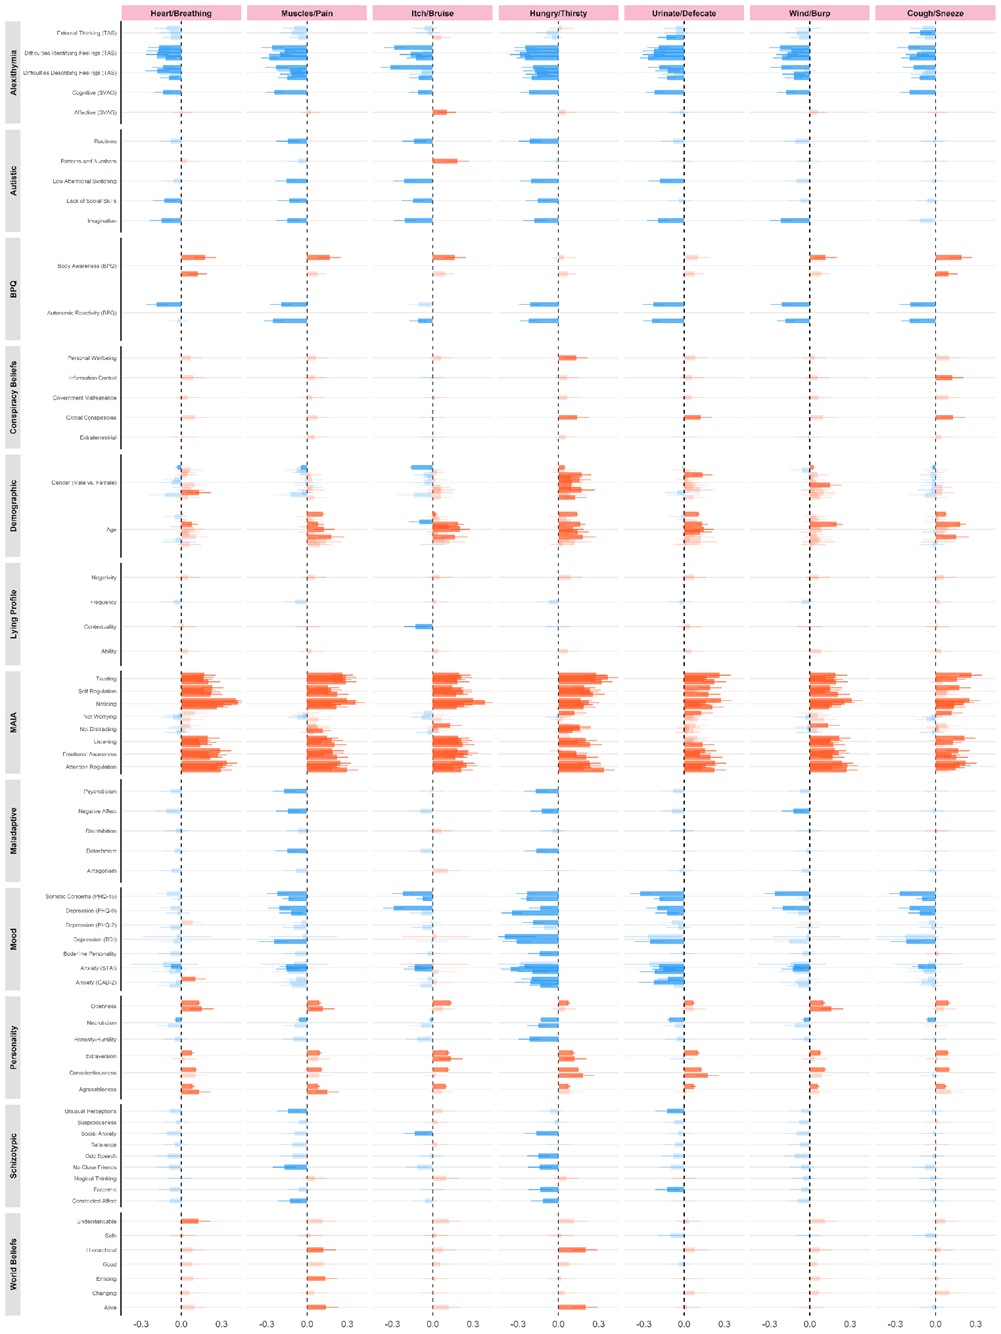
\includegraphics[width=9.48958in,height=\textheight]{figures/clipboard-1619164537.png}

}

\end{figure}%

\subsubsection{Discussion}\label{discussion-1}

Our findings confirmed that interception lies within an intricate
network of correlates. Alexithyma has the most negative correlation with
the IAS, whereas, the MAIA questionnaire is most strongly positively
correlated with the IAS. The correlates cannot only explain attributes
of interoception, but can also be used to validate measures for
interoception.

While these results reveal correlations of different categories with the
IAS, the findings are limited to the given questionnaire. However, they
give a good indication of how interoception in general might be linked
to the different categories, leading to interesting findings. The
results show a consistent pattern of correlations with other
interoception measures, psychopathology, and highlighting of interesting
exploratory results, such as how primal world beliefs correlate with the
IAS.

The analysis revealed a negative correlation between alexithymia and
scores in the IAS, which is in line with previous research
(\citeproc{ref-herbert2011}{Herbert et al., 2011}). A negative
correlation between autism and interoceptive awareness, which has been
found in this sample, has also been found in previous research
(\citeproc{ref-dubois2016}{DuBois et al., 2016}). Conspiracy Beliefs and
IAS scores were not strongly correlated. However, there was a slight
positive correlation. To the best of our knowledge, this interaction has
not been investigated before. However, research shows correlations
between (political) beliefs and interoception, which could underlie the
same mechanism (\citeproc{ref-ruisch2022}{Ruisch et al., 2022a}). Lying
profile was also not strongly correlated with the IAS. Previous research
provides some evidence for a relationshipbetween interoception and lying
profile (\citeproc{ref-makowski2023a}{Makowski et al., 2023}),
indicating a contrast from the literature to the results at hand. The
analysis showed that mood and the IAS scores have a strong negative
correlation, which has been investigated in previous studies, finding a
correlation between the two variables as well
(\citeproc{ref-solanoluxf3pez2018}{Solano López \& Moore, 2018}). The
analysis showed that personality is also correlated with interoceptive
accuracy scores as retrieved by the IAS. While there are many aspects of
personality, put simply, personality and interoception have been found
to correlate in previous studies as well (\citeproc{ref-erle2021}{Erle
et al., 2021}). Our findings show some negative correlations between
schizotypy and interoception. Previous research has investigated this
relationship and, similarly, found a negative correlation between
interoceptive awareness and schizotypy, particularly at the onset of
psychosis (\citeproc{ref-torregrossa2022}{Torregrossa et al., 2022}).
Lastly, World Beliefs and Interoception showed some significant positive
correlations. World Beliefs have not been linked with interoception
previously. As mentioned, other beliefs, such as political beliefs have
been mentioned to interoception, where significant correlations were
observed (\citeproc{ref-ruisch2022a}{Ruisch et al., 2022b}). Further
research is needed to understand this mechanism and validate whether
world beliefs, which lay the framework through which we see the world
(\citeproc{ref-clifton2020}{Clifton, 2020}), is needed.

The above findings show how interoception is correlated with many
lifestyle and health factors, and is therefore an important concept to
study. Here we showed many correlates of the IAS and lifestyle, as well
as health factors. This is not only valuable to understand interception,
and the role it plays in our lives, better, but also crucial to further
validate the Ias, as well as other interoception measures. This analysis
therefore lays the groundwork for validating new interoceptive measures
and questionnaires needed to grasp interoception and its role in our
life.

\subsection{General Discussion}\label{general-discussion}

The analyses revealed that the IAS has 4-factor structure, and a rather
uneven distribution. The findings indicate that the IAS is measuring
interoception in an acceptable manner, but there is also room for
improvement. Furthermore, the results reveal different correlation
measures with the IAS, giving space to further explore whether and how
measures correlate with interoception/the IAS. In the following section,
the IAS is discussed further to reveal shortcomings and strengths of the
questionnaire. Finally, future steps will be revealed to improve the way
in which we measure interoception.

Overall, the IAS is straightforward with its sensation-centered items.
There are several points of improvement to the IAS, which this work
suggests. Firstly, removing redundant items, such as the itch item as
shown in the above analysis. Previous work has also shown that the itch
and tickle items are subject to redundancy Campos et al.
(\citeproc{ref-campos2021}{2021}) has shown. Interestingly, Campos et
al. (\citeproc{ref-campos2021}{2021}) suggest removing the tickle item
instead. Lin et al. (\citeproc{ref-lin2023}{2023}) on the other hand
removed the itch item, because the sign for itch and tickle is the same.
Furthermore, this work recommends using analog scales, instead of 5
point scales. In a 5-point scale, the variability is clearly limited
with most people choosing ⅘. As visible in Figure X, the variability
increases significantly, using an analog scale. However, it is important
to note that even with an analog scale, the variability of the IAS is
still limited. The more variability a scale shows, the more results can
depict individual differences between participants. Therefore, good
dispersion is essential for achieving relevant and usable results, and
striving for more variability would be beneficial to this interoception
scale, too.

In this work, it becomes apparent that even with the mentioned
improvements to the scale, there are limitations to the IAS, which
reduce the accuracy of this scale. Those limitations include that there
are few items for some modalities, such as only one item for heart
perception. Having more modality is useful as each grouping can have
more variability with increased modality, leading to more nuanced
results. On top of that, there is no clear and theoretical, or empirical
structure, as there is a very small grouping of items. Ideally, a scale
would allow for an analysis showing different groupings so that
different categories can be created based on which the data can be
analyzed. The groupings in this analysis reveal that the IAS can only be
grouped with two items per group, leading to low scores and variability
in each group. On top of that, there are ambiguous items in the IAS, of
which the grouping depends on the context. For example, one might
indicate that they can perceive well how their heart is beating fast as
well as vomiting, but both items can be linked to feeling anxious, and
therefore might indicate different results than initially expected.
Therefore, the grouping and structure of the IAS can be improved.

Furthermore, all items are phrased positively, which might influence how
participants answer the questions. While phrasing items in a positive
manner can be beneficial, the benefits of positive phrasing might
exacerbate a positive bias and thus lead to unidimensional results.
Therefore, phrasing questions in a more diverse manner might lead to
more accurate results and might thus be beneficial.

Based on the given arguments, it becomes clear that there is a need for
context-specific items, which are cross-modal when possible, such as
integrating cardioception and respiroception. After establishing the
clear need for a new scale to measure interoception, this study proposes
the need for a new scale (Multimodal Interoceptive Sensitivity Scale,
MISS) to adapt to the newest findings on the IAS and what we know about
interoception to this day. The new scale will be able to be compared to
the correlates of the IAS.

\subsection{Conclusion}\label{conclusion}

The IAS is a good way of measuring interoception considering the current
existing questionnaires and tools. However, revising, or even
re-inventing a survey to measure interoception would lead to the best
measure of interoception. Therefore, this study proposes that a new
scale to measure interoception is needed to evolve the current research
on interoception. This study revealed many correlates of the IAS, giving
space for future analysis on what might be a good interoceptive measure,
and therefore laying the groundwork for the creation of a new
interoception survey.

{[}\textbf{TO DO}: add - previous work suggests the importance of
physiological contexts (Vlemincx et al., 2021){]} \textbf{I would rather
put that in the discussion in the suggestions for better scales}

\subsection{References}\label{references}

\phantomsection\label{refs}
\begin{CSLReferences}{1}{0}
\bibitem[\citeproctext]{ref-arslanova2022}
Arslanova, I., Galvez-Pol, A., Kilner, J., Finotti, G., \& Tsakiris, M.
(2022). Seeing through each other's hearts: Inferring others' heart rate
as a function of own heart rate perception and perceived social
intelligence. \emph{Affective Science}, \emph{3}(4), 862--877.

\bibitem[\citeproctext]{ref-baer2006using}
Baer, R. A., Smith, G. T., Hopkins, J., Krietemeyer, J., \& Toney, L.
(2006). Using self-report assessment methods to explore facets of
mindfulness. \emph{Assessment}, \emph{13}(1), 27--45.

\bibitem[\citeproctext]{ref-brand2023}
Brand, S., Meis, A. C., Tünte, M. R., Murphy, J., Woller, J. P.,
Jungmann, S. M., Witthöft, M., Hoehl, S., Weymar, M., Hermann, C., \&
Ventura-Bort, C. (2023). A multi-site German validation of the
Interoceptive Accuracy Scale and its relation to psychopathological
symptom burden. \emph{Communications Psychology}, \emph{1}(1).
\url{https://doi.org/10.1038/s44271-023-00016-x}

\bibitem[\citeproctext]{ref-brand2022}
Brand, S., Petzke, T. M., \& Witthöft, M. (2022). The differential
relationship between self-reported interoceptive accuracy and attention
with psychopathology. \emph{Zeitschrift f{ü}r Klinische Psychologie Und
Psychotherapie}.

\bibitem[\citeproctext]{ref-brewer2016alexithymia}
Brewer, R., Cook, R., \& Bird, G. (2016). Alexithymia: A general deficit
of interoception. \emph{Royal Society Open Science}, \emph{3}(10),
150664.

\bibitem[\citeproctext]{ref-campos2021}
Campos, C., Rocha, N. B., \& Barbosa, F. (2021). \emph{Untangling
self-reported interoceptive attention and accuracy: Evidence from the
european portuguese validation of the body perception questionnaire and
the interoceptive accuracy scale}.
\url{http://dx.doi.org/10.31234/osf.io/a7wdj}

\bibitem[\citeproctext]{ref-christensen2023unique}
Christensen, A. P., Garrido, L. E., \& Golino, H. (2023). Unique
variable analysis: A network psychometrics method to detect local
dependence. \emph{Multivariate Behavioral Research}, \emph{58}(6),
1165--1182.

\bibitem[\citeproctext]{ref-christensen2021}
Christensen, A. P., \& Golino, H. (2021). Estimating the Stability of
Psychological Dimensions via Bootstrap Exploratory Graph Analysis: A
Monte Carlo Simulation and Tutorial. \emph{Psych}, \emph{3}(3),
479--500. \url{https://doi.org/10.3390/psych3030032}

\bibitem[\citeproctext]{ref-clifton2020}
Clifton, J. D. W. (2020). Testing if primal world beliefs reflect
experiences{\textemdash}or at least some experiences identified ad hoc.
\emph{Frontiers in Psychology}, \emph{11}.
\url{https://doi.org/10.3389/fpsyg.2020.01145}

\bibitem[\citeproctext]{ref-desmedt2022measures}
Desmedt, O., Heeren, A., Corneille, O., \& Luminet, O. (2022). What do
measures of self-report interoception measure? Insights from a
systematic review, latent factor analysis, and network approach.
\emph{Biological Psychology}, \emph{169}, 108289.

\bibitem[\citeproctext]{ref-dubois2016}
DuBois, D., Ameis, S. H., Lai, M.-C., Casanova, M. F., \& Desarkar, P.
(2016). Interoception in Autism Spectrum Disorder: A review.
\emph{International Journal of Developmental Neuroscience},
\emph{52}(1), 104--111.
\url{https://doi.org/10.1016/j.ijdevneu.2016.05.001}

\bibitem[\citeproctext]{ref-erle2021}
Erle, T. M., Mitschke, V., \& Schultchen, D. (2021). Did my heart just
leap or sink? The role of personality for the relation between cardiac
interoception and well-being. \emph{Personality and Individual
Differences}, \emph{170}, 110493.
\url{https://doi.org/10.1016/j.paid.2020.110493}

\bibitem[\citeproctext]{ref-gabriele2022dissociations}
Gabriele, E., Spooner, R., Brewer, R., \& Murphy, J. (2022).
Dissociations between self-reported interoceptive accuracy and
attention: Evidence from the interoceptive attention scale.
\emph{Biological Psychology}, \emph{168}, 108243.

\bibitem[\citeproctext]{ref-gaggero2021}
Gaggero, G., Bizzego, A., Dellantonio, S., Pastore, L., Lim, M., \&
Esposito, G. (2021). Clarifying the relationship between alexithymia and
subjective interoception. \emph{PLoS One}, \emph{16}(12), e0261126.

\bibitem[\citeproctext]{ref-garfinkel2015knowing}
Garfinkel, S. N., Seth, A. K., Barrett, A. B., Suzuki, K., \& Critchley,
H. D. (2015). Knowing your own heart: Distinguishing interoceptive
accuracy from interoceptive awareness. \emph{Biological Psychology},
\emph{104}, 65--74.

\bibitem[\citeproctext]{ref-golino2017exploratory}
Golino, H. F., \& Epskamp, S. (2017). Exploratory graph analysis: A new
approach for estimating the number of dimensions in psychological
research. \emph{PloS One}, \emph{12}(6), e0174035.

\bibitem[\citeproctext]{ref-herbert2011}
Herbert, B. M., Herbert, C., \& Pollatos, O. (2011). On the Relationship
Between Interoceptive Awareness and Alexithymia: Is Interoceptive
Awareness Related to Emotional Awareness? \emph{Journal of Personality},
\emph{79}(5), 1149--1175.
\url{https://doi.org/10.1111/j.1467-6494.2011.00717.x}

\bibitem[\citeproctext]{ref-jahedi2014}
Jahedi, S., \& Méndez, F. (2014). On the advantages and disadvantages of
subjective measures. \emph{Journal of Economic Behavior \&
Organization}, \emph{98}, 97--114.
\url{https://doi.org/10.1016/j.jebo.2013.12.016}

\bibitem[\citeproctext]{ref-khalsa2018}
Khalsa, S. S., Adolphs, R., Cameron, O. G., Critchley, H. D., Davenport,
P. W., Feinstein, J. S., Feusner, J. D., Garfinkel, S. N., Lane, R. D.,
Mehling, W. E., Meuret, A. E., Nemeroff, C. B., Oppenheimer, S.,
Petzschner, F. H., Pollatos, O., Rhudy, J. L., Schramm, L. P., Simmons,
W. K., Stein, M. B., \ldots{} Zucker, N. (2018). Interoception and
Mental Health: A Roadmap. \emph{Biological Psychiatry: Cognitive
Neuroscience and Neuroimaging}, \emph{3}(6), 501--513.
\url{https://doi.org/10.1016/j.bpsc.2017.12.004}

\bibitem[\citeproctext]{ref-koike2023}
Koike, H., \& Nomura, M. (2023). Development and validation of japanese
versions of the interoceptive accuracy scale and interoceptive attention
scale. \emph{SAGE Open}, \emph{13}(4), 21582440231214639.

\bibitem[\citeproctext]{ref-lin2023}
Lin, X.-X., Shen, H.-R., Lin, J.-X., Zhang, Y.-H., Murphy, J., Wang,
Y.-Z., Sun, Y.-B., Wang, N., Wang, J.-Y., Wei, G.-X., \& Luo, F. (2023).
Psychometric validation and refinement of the Chinese Interoceptive
Accuracy Scale (IAS) in general population and patients with chronic
pain. \emph{Journal of Psychosomatic Research}, \emph{175}, 111541.
\url{https://doi.org/10.1016/j.jpsychores.2023.111541}

\bibitem[\citeproctext]{ref-makowski2023a}
Makowski, D., Lau, Z. J., Pham, T., Te, A., Kirk, S., \& Liauw Yong
Tong, C. (2023). \emph{The heart can lie: The role of interoception and
theory of mind in deception}.
\url{http://dx.doi.org/10.31234/osf.io/p342w}

\bibitem[\citeproctext]{ref-mehling2018multidimensional}
Mehling, W. E., Acree, M., Stewart, A., Silas, J., \& Jones, A. (2018).
The multidimensional assessment of interoceptive awareness, version 2
(MAIA-2). \emph{PloS One}, \emph{13}(12), e0208034.

\bibitem[\citeproctext]{ref-mehling2012}
Mehling, W. E., Price, C., Daubenmier, J. J., Acree, M., Bartmess, E.,
\& Stewart, A. (2012). The Multidimensional Assessment of Interoceptive
Awareness (MAIA). \emph{PLoS ONE}, \emph{7}(11), e48230.
\url{https://doi.org/10.1371/journal.pone.0048230}

\bibitem[\citeproctext]{ref-murphy2019}
Murphy, J., Brewer, R., Plans, D., Khalsa, S. S., Catmur, C., \& Bird,
G. (2019). Testing the independence of self-reported interoceptive
accuracy and attention. \emph{Quarterly Journal of Experimental
Psychology}, \emph{73}(1), 115--133.
\url{https://doi.org/10.1177/1747021819879826}

\bibitem[\citeproctext]{ref-porges1993body}
Porges, S. (1993). Body perception questionnaire. \emph{Laboratory of
Developmental Assessment, University of Maryland}, \emph{10},
s15327752jpa5304\_1.

\bibitem[\citeproctext]{ref-rodriguez2016evaluating}
Rodriguez, A., Reise, S. P., \& Haviland, M. G. (2016). Evaluating
bifactor models: Calculating and interpreting statistical indices.
\emph{Psychological Methods}, \emph{21}(2), 137.

\bibitem[\citeproctext]{ref-ruisch2022}
Ruisch, B. C., Von Mohr, M., Naber, M., Tsakiris, M., Fazio, R. H., \&
Scheepers, D. T. (2022a). Sensitive liberals and unfeeling
conservatives? {\emph{Interoceptive sensitivity predicts political
liberalism}}. \emph{Politics and the Life Sciences}, \emph{41}(2),
256--275. \url{https://doi.org/10.1017/pls.2022.18}

\bibitem[\citeproctext]{ref-ruisch2022a}
Ruisch, B. C., Von Mohr, M., Naber, M., Tsakiris, M., Fazio, R. H., \&
Scheepers, D. T. (2022b). Sensitive liberals and unfeeling
conservatives? {\emph{Interoceptive sensitivity predicts political
liberalism}}. \emph{Politics and the Life Sciences}, \emph{41}(2),
256--275. \url{https://doi.org/10.1017/pls.2022.18}

\bibitem[\citeproctext]{ref-solanoluxf3pez2018}
Solano López, A. L., \& Moore, S. (2018). Dimensions of Body-Awareness
and Depressed Mood and Anxiety. \emph{Western Journal of Nursing
Research}, \emph{41}(6), 834--853.
\url{https://doi.org/10.1177/0193945918798374}

\bibitem[\citeproctext]{ref-todd2022}
Todd, J., Swami, V., Aspell, J. E., Furnham, A., Horne, G., \& Stieger,
S. (2022). Are some interoceptive sensibility components more central
than others? Using item pool visualisation to understand the
psychometric representation of interoception. \emph{Plos One},
\emph{17}(12), e0277894.

\bibitem[\citeproctext]{ref-torregrossa2022}
Torregrossa, L. J., Amedy, A., Roig, J., Prada, A., \& Park, S. (2022).
Interoceptive functioning in schizophrenia and schizotypy.
\emph{Schizophrenia Research}, \emph{239}, 151--159.
\url{https://doi.org/10.1016/j.schres.2021.11.046}

\bibitem[\citeproctext]{ref-von2023}
Von Mohr, M., Silva, P. C., Vagnoni, E., Bracher, A., Bertoni, T.,
Serino, A., Banissy, M. J., Jenkinson, P. M., \& Fotopoulou, A. (2023).
My social comfort zone: Attachment anxiety shapes peripersonal and
interpersonal space. \emph{Iscience}, \emph{26}(2).

\end{CSLReferences}






\end{document}
